\def \currentAuthor {Florian Tipotsch}

\section{Webapp}

Für unser Projekt erstellen wir eine Webapp mit der man die Daten seiner eigenen Zuchtkammer anzeigen lassen kann.
Wir haben geplant das man sich mit der Seriennummer der Box Registrieren kann und dann am Handy über eine Webapp alle Daten anzeigen lassen kann. Folgende Daten sollte man auslesen können:

\begin{itemize}
	\item Sauerstoff
	\item Luftfeuchtigkeit
	\item Gewicht
	\item Temperatur
	\item Futtermenge
	\item ungefähre Zeit bis zu Reife
\end{itemize}
Als Grundlage für die Website haben wir das Framework Yii2 verwendet. Mehr dazu im Kapitel \nameref{sec:YII2}.

\subsection{Mockups}
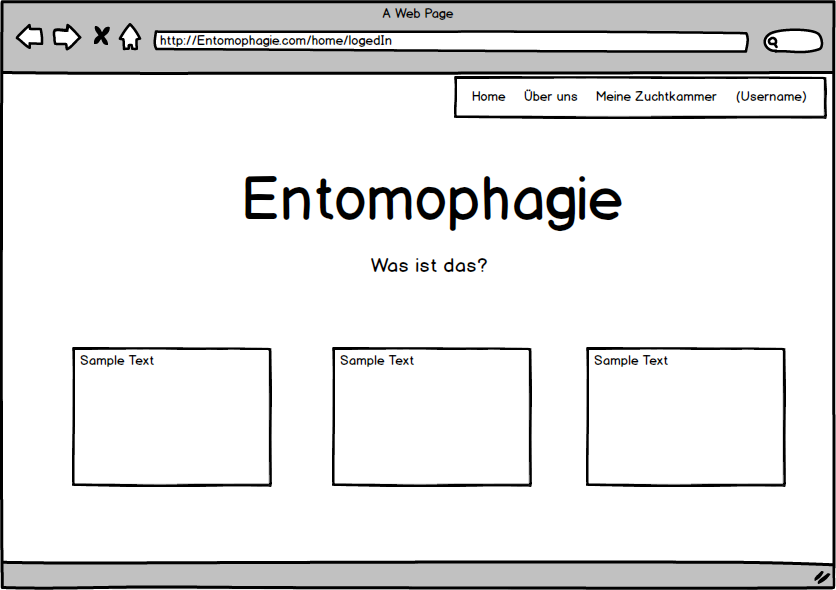
\includegraphics[height=10cm]{figures/Logedin}
Hier sieht man die Ansicht wenn man auf unserer Website Angemeldet ist. Man kann auf seine eigene Zuchtkammer zugreifen indem man auf den Button "Meine Zuchtkammer" klickt und dort die Daten auslesen.
\newpage
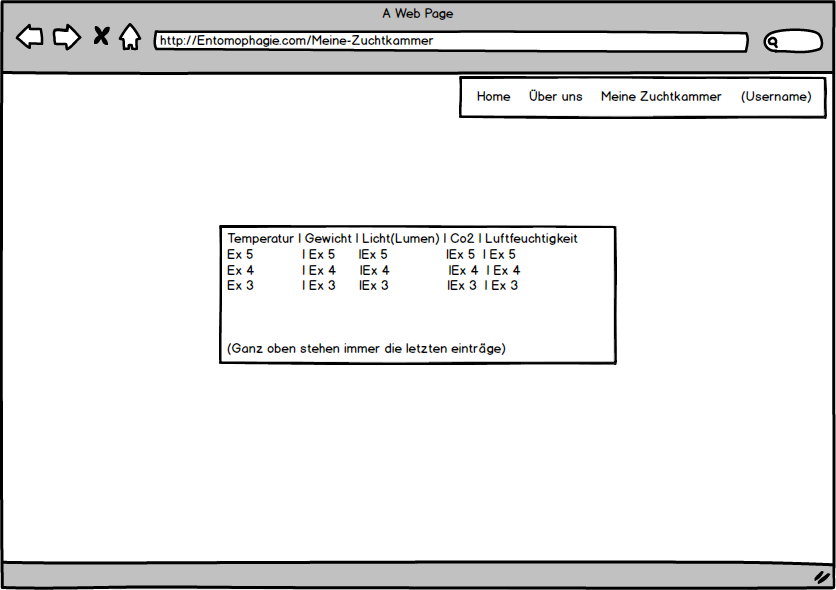
\includegraphics[height=10cm]{figures/Meine-Zuchtkammer}
Auf der Seite "Meine Zuchtkammer" sieht die letzten 10 Daten die meine Zuchtkammer wiedergegeben hat. Diese sind in Absteigender Reihenfolge geordnet,dass heißt, dass der letzte Eintrag ganz oben steht.
\newpage
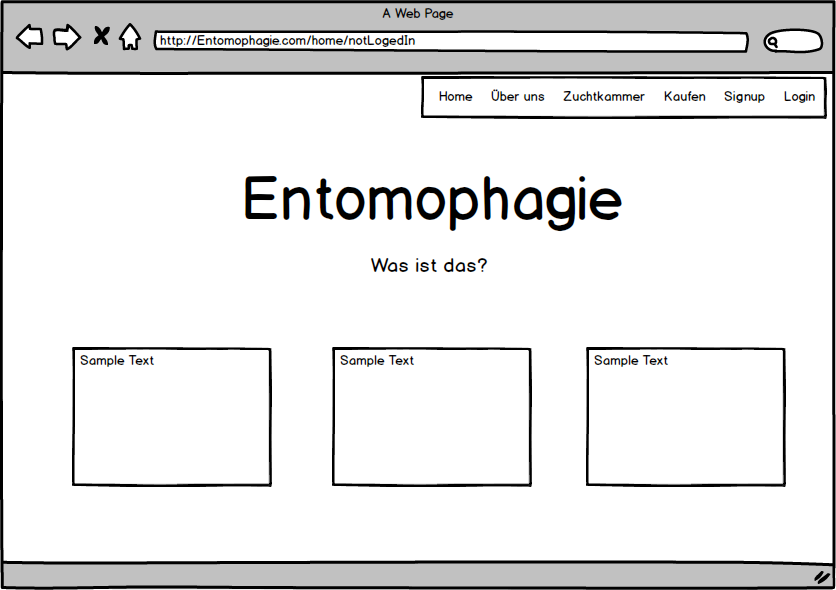
\includegraphics[height=10cm]{figures/NotlogedIN}
Hier Sieht man die Ansicht wenn man auf unserer Website nicht Angemeldet ist. Man kann über den Button "Zuchtkammer" mehr über unsere Zuchtkammern herausfinden, weiter kann man über den Button "Kaufen" seine eigene Zuchtkammer kaufen. Bei Signup kann man sich als neuer Benutzer registrieren, um sich allerdings zu registrieren brauch man zuerst eine Seriennummer die man beim kauf einer Zuchtkammer erhält.
\newpage

\subsection{Datenbankzugriffe}
Unserer Datenbank zugriffe werden von unserem Framework verarbeite, dabei verwendet das Framework CRUD befehle und nach dem MVC Muster. Das heißt es gibt ein unterliegendes Modell welches Daten unserem Controller mitgibt welche wiederum die View erzeugt.

Der gesamte Datenbankzugriff kann mittels Yii2 sehr einfach erstellt werden. Mehr dazu siehe \nameref{sec:gii}